\documentclass[default]{beamer}
\setbeamertemplate{navigation symbols}{}

\usetheme{CambridgeUS}
\useoutertheme{infolines}
%\usecolortheme{crane}

\usepackage[utf8]{inputenc}					% Выбор языка и кодировки
\usepackage{tikz}
\usepackage{animate}
\usepackage{fp}

\usetikzlibrary{calc,patterns,backgrounds}

\graphicspath{{../../images/}} 			% Пути к изображениям

\makeatletter
\setbeamertemplate{footline}
{
	\leavevmode%
	\hbox{%
		\begin{beamercolorbox}[wd=.333333\paperwidth,ht=2.25ex,dp=1ex,center]{author
				in head/foot}%
			\usebeamerfont{author in
				head/foot}\insertshortauthor~~\beamer@ifempty{\insertshortinstitute}{}{(\insertshortinstitute)}
		\end{beamercolorbox}%
		\begin{beamercolorbox}[wd=.333333\paperwidth,ht=2.25ex,dp=1ex,center]{title in
				head/foot}%
			\usebeamerfont{title in head/foot}\insertshorttitle
		\end{beamercolorbox}%
		\begin{beamercolorbox}[wd=.333333\paperwidth,ht=2.25ex,dp=1ex,right]{date in
				head/foot}%
			\usebeamerfont{date in head/foot}\insertshortdate{}\hspace*{2em}
			\insertframenumber{}\hspace*{2ex} 
		\end{beamercolorbox}
	}%
	\vskip0pt%
}

\begin{document}
	
	\title[RiTA'2015 -- Behavior and path planning]{Behavior and path planning for the coalition of cognitive robots in smart relocation tasks}
	\author[Panov, Yakovlev]{Aleksandr Panov, Konstantin Yakovlev}
	
	\institute[FRC CSC]{Lab ``Dynamic Intelligent Systems''\\
		Institute for Systems Analysis of Federal Research Center ``Computer Science and Control''\\
		\textbf{Russian Academy of Sciences}}
	\date{December 15, 2015} 
	
	\begin{frame}
		\titlepage
	\end{frame}
	
	\begin{frame}
		\frametitle{Authors' origin}
		\begin{tikzpicture}
			
		\end{tikzpicture}
				
		\begin{columns}
			\begin{column}{0.5\textwidth}
				\centering
				\begin{tikzpicture}
					\node[anchor=south west,inner sep=0] at (0,0) {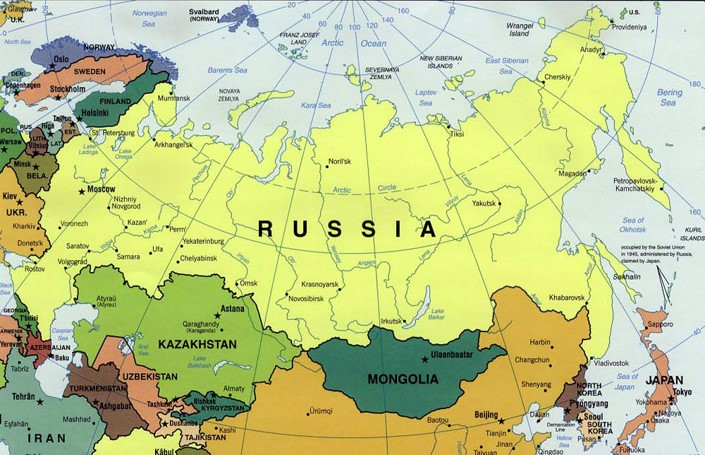
\includegraphics[width=\textwidth]{misc/origin_russia.jpg}};
					\draw[red,ultra thick] (0.75,2.25) circle (2mm);
				\end{tikzpicture}
				\par\bigskip
				
\includegraphics[width=0.4\textwidth]{misc/origin_flag.png}
			\end{column}
			\begin{column}{0.5\textwidth}
				\centering
				
\includegraphics[width=0.3\textwidth]{misc/origin_gerb.png}
				\par\bigskip
				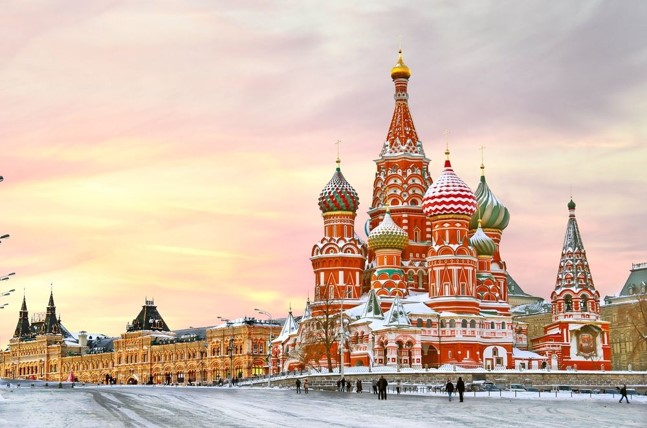
\includegraphics[width=\textwidth]{misc/origin_moscow.jpg}
			\end{column}
		\end{columns}

	\end{frame}
	
	\begin{frame}
		\frametitle{Authors' background}
		
		\begin{columns}
			\begin{column}{0.5\textwidth}
				Federal Research Centre ``Computer Science and Control'' of \textbf{Russian Academy of Sciences}
				\par\bigskip
				\textbf{Research interests}: Artificial Intelligence, Cognitive Modeling, Semiotics, Task Planning, Heuristic Search, Path Planning, Robotics
				\par\bigskip
				\textbf{Ongoing research}: Multilayered cognitive architecture of the control system for intelligent agents (including mobile robots, UAVs, etc.) -- \textbf{STRL architecture}
				
			\end{column}
			\begin{column}{0.5\textwidth}
				\centering
				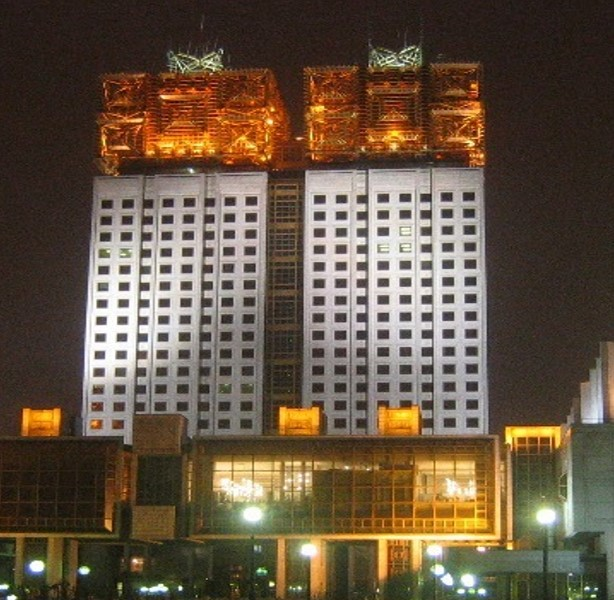
\includegraphics[width=\textwidth]{misc/origin_ras.jpg}
			\end{column}
		\end{columns}
		
	\end{frame}
		
	\begin{frame}
		\frametitle{STRL architecture}
		
		\begin{columns}
			\begin{column}{0.6\textwidth}
				\centering
				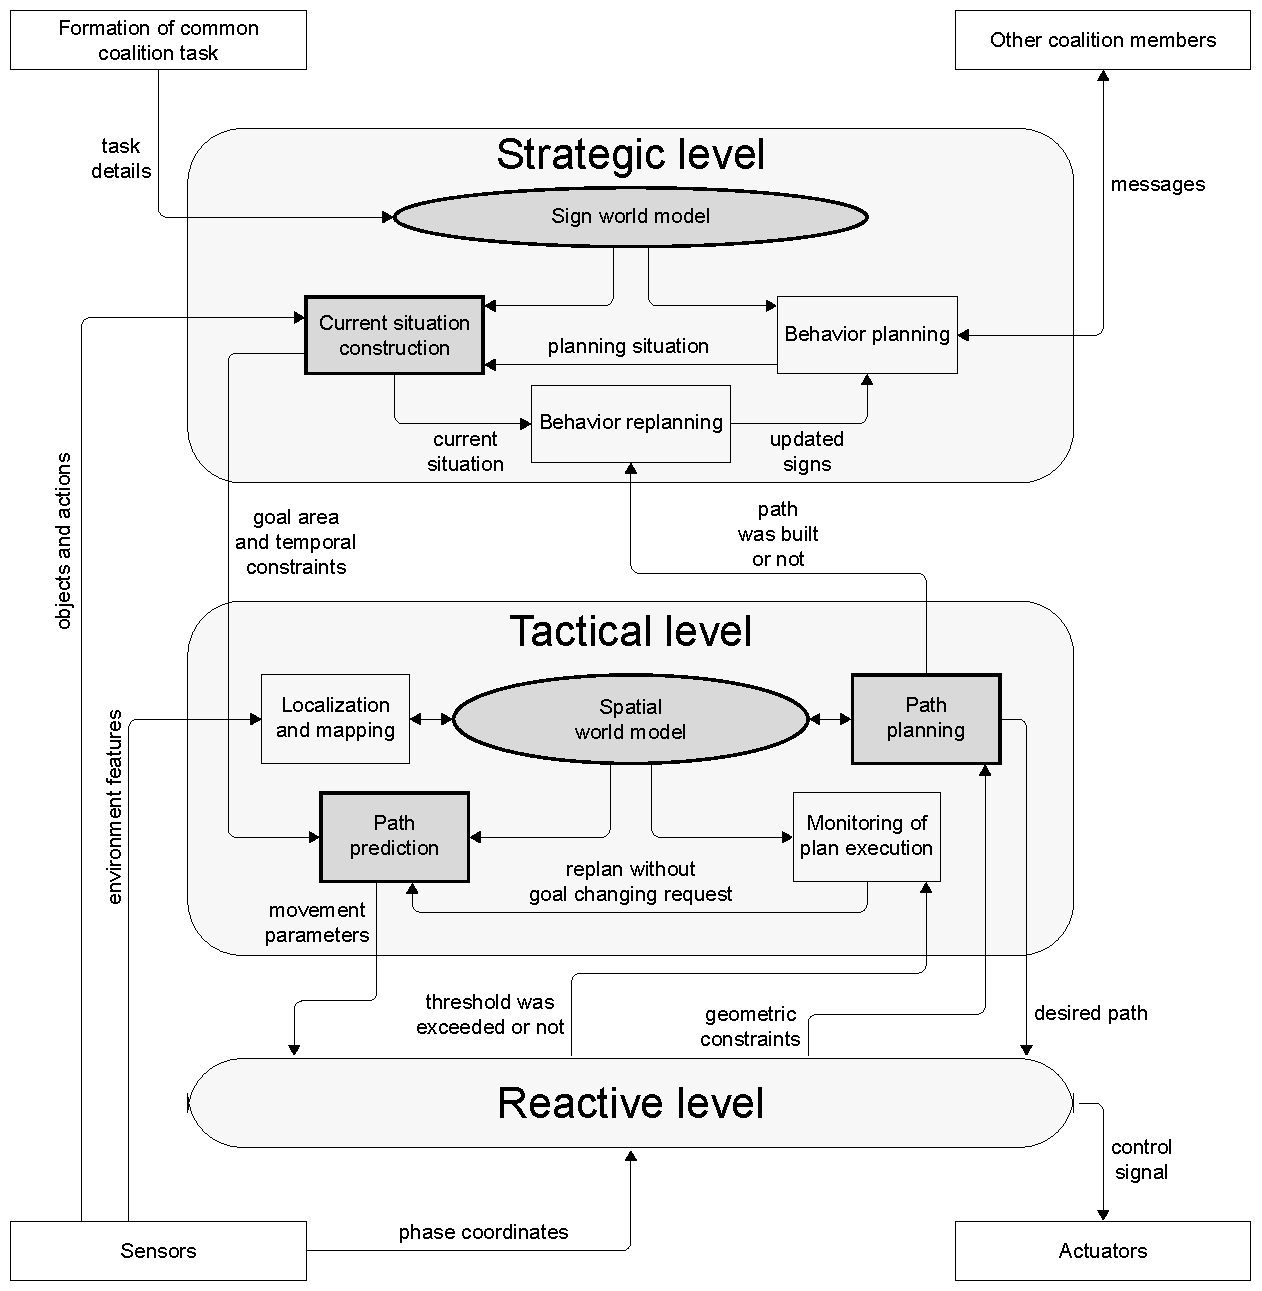
\includegraphics[width=\textwidth]{strl/strl_rita_eng}
			\end{column}
			\begin{column}{0.4\textwidth}
				3 levels of control:
				\begin{itemize}
					\item \textbf{Strategic}: Behavior planning (including inter-agent communication
					\item \textbf{Tactic}: Path planning (including prediction and monitoring)
					\item \textbf{Reactive}: Path following taking into account agent’s dynamic
				\end{itemize}
			\end{column}
		\end{columns}
	\end{frame}

	\begin{frame}
		\frametitle{Smart Relocation Tasks (SRT)}
		
		\begin{columns}
			\begin{column}{0.55\textwidth}
				\begin{center}
					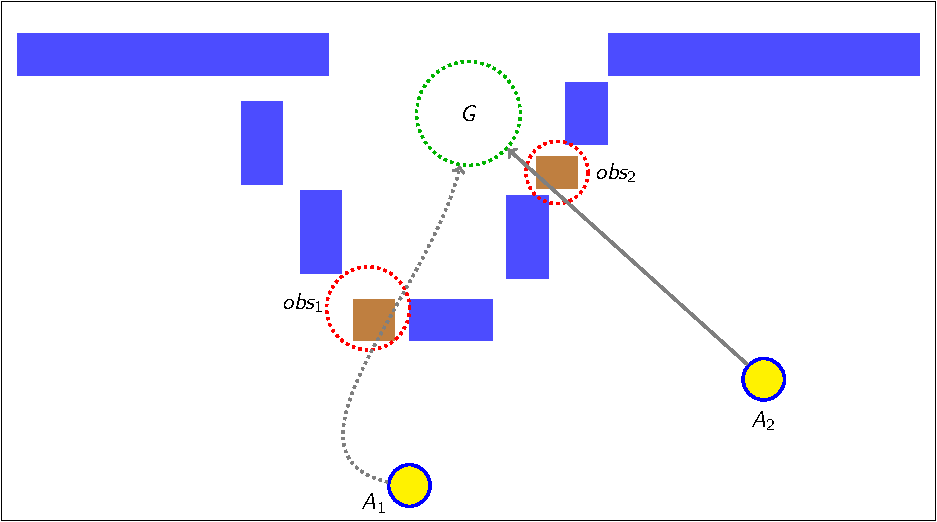
\includegraphics[page=1,width=0.85\textwidth]{slides_colored}
				\end{center}
				
				\textbf{Problem}
				
				Goal area can not be achieved by some agents on their own (using standalone task and path planning methods)
				
				\textbf{Solution}
				
				Agents must communicate and some agents must alter their ``selfish'' plans in order to construct coalition plan
				
			\end{column}
			\begin{column}{0.45\textwidth}
				3 levels of control:
				\begin{itemize}
					\item Transformable environment
					\item Different types of obstacles (some -- can be destroyed)
					\item Agents with different capabilities (some agents can destroy obstacles, others -- can not)
					\item Common spatial goal (ALL agents must reach this region in order goal to be achieved)
				\end{itemize}
			\end{column}
		\end{columns}
	\end{frame}
			
	\begin{frame}
		\frametitle{Plan execution}
		\begin{center}
			\scalebox{0.7}{
				\animategraphics{12}{slides_colored}{}{}			
			}
		\end{center}
	\end{frame}		

	\begin{frame}
		\frametitle{Sign knowledge representation}
		
		Sign as a component of knowledge:
		\begin{itemize}
			\item cultural-historical approach of Vygotsky-Luria
			\item the theory of activity of Leontiev
		\end{itemize}
		
		\begin{columns}
			\begin{column}{0.4\textwidth}
				\centering
				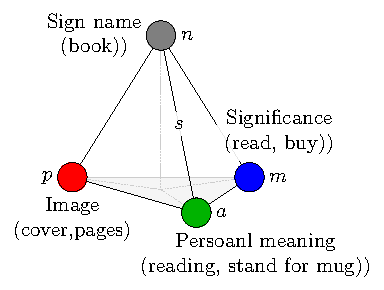
\includegraphics[width=\textwidth]{signs/sign_colored_rita.pdf}
			\end{column}
			\begin{column}{0.6\textwidth}
				\centering
				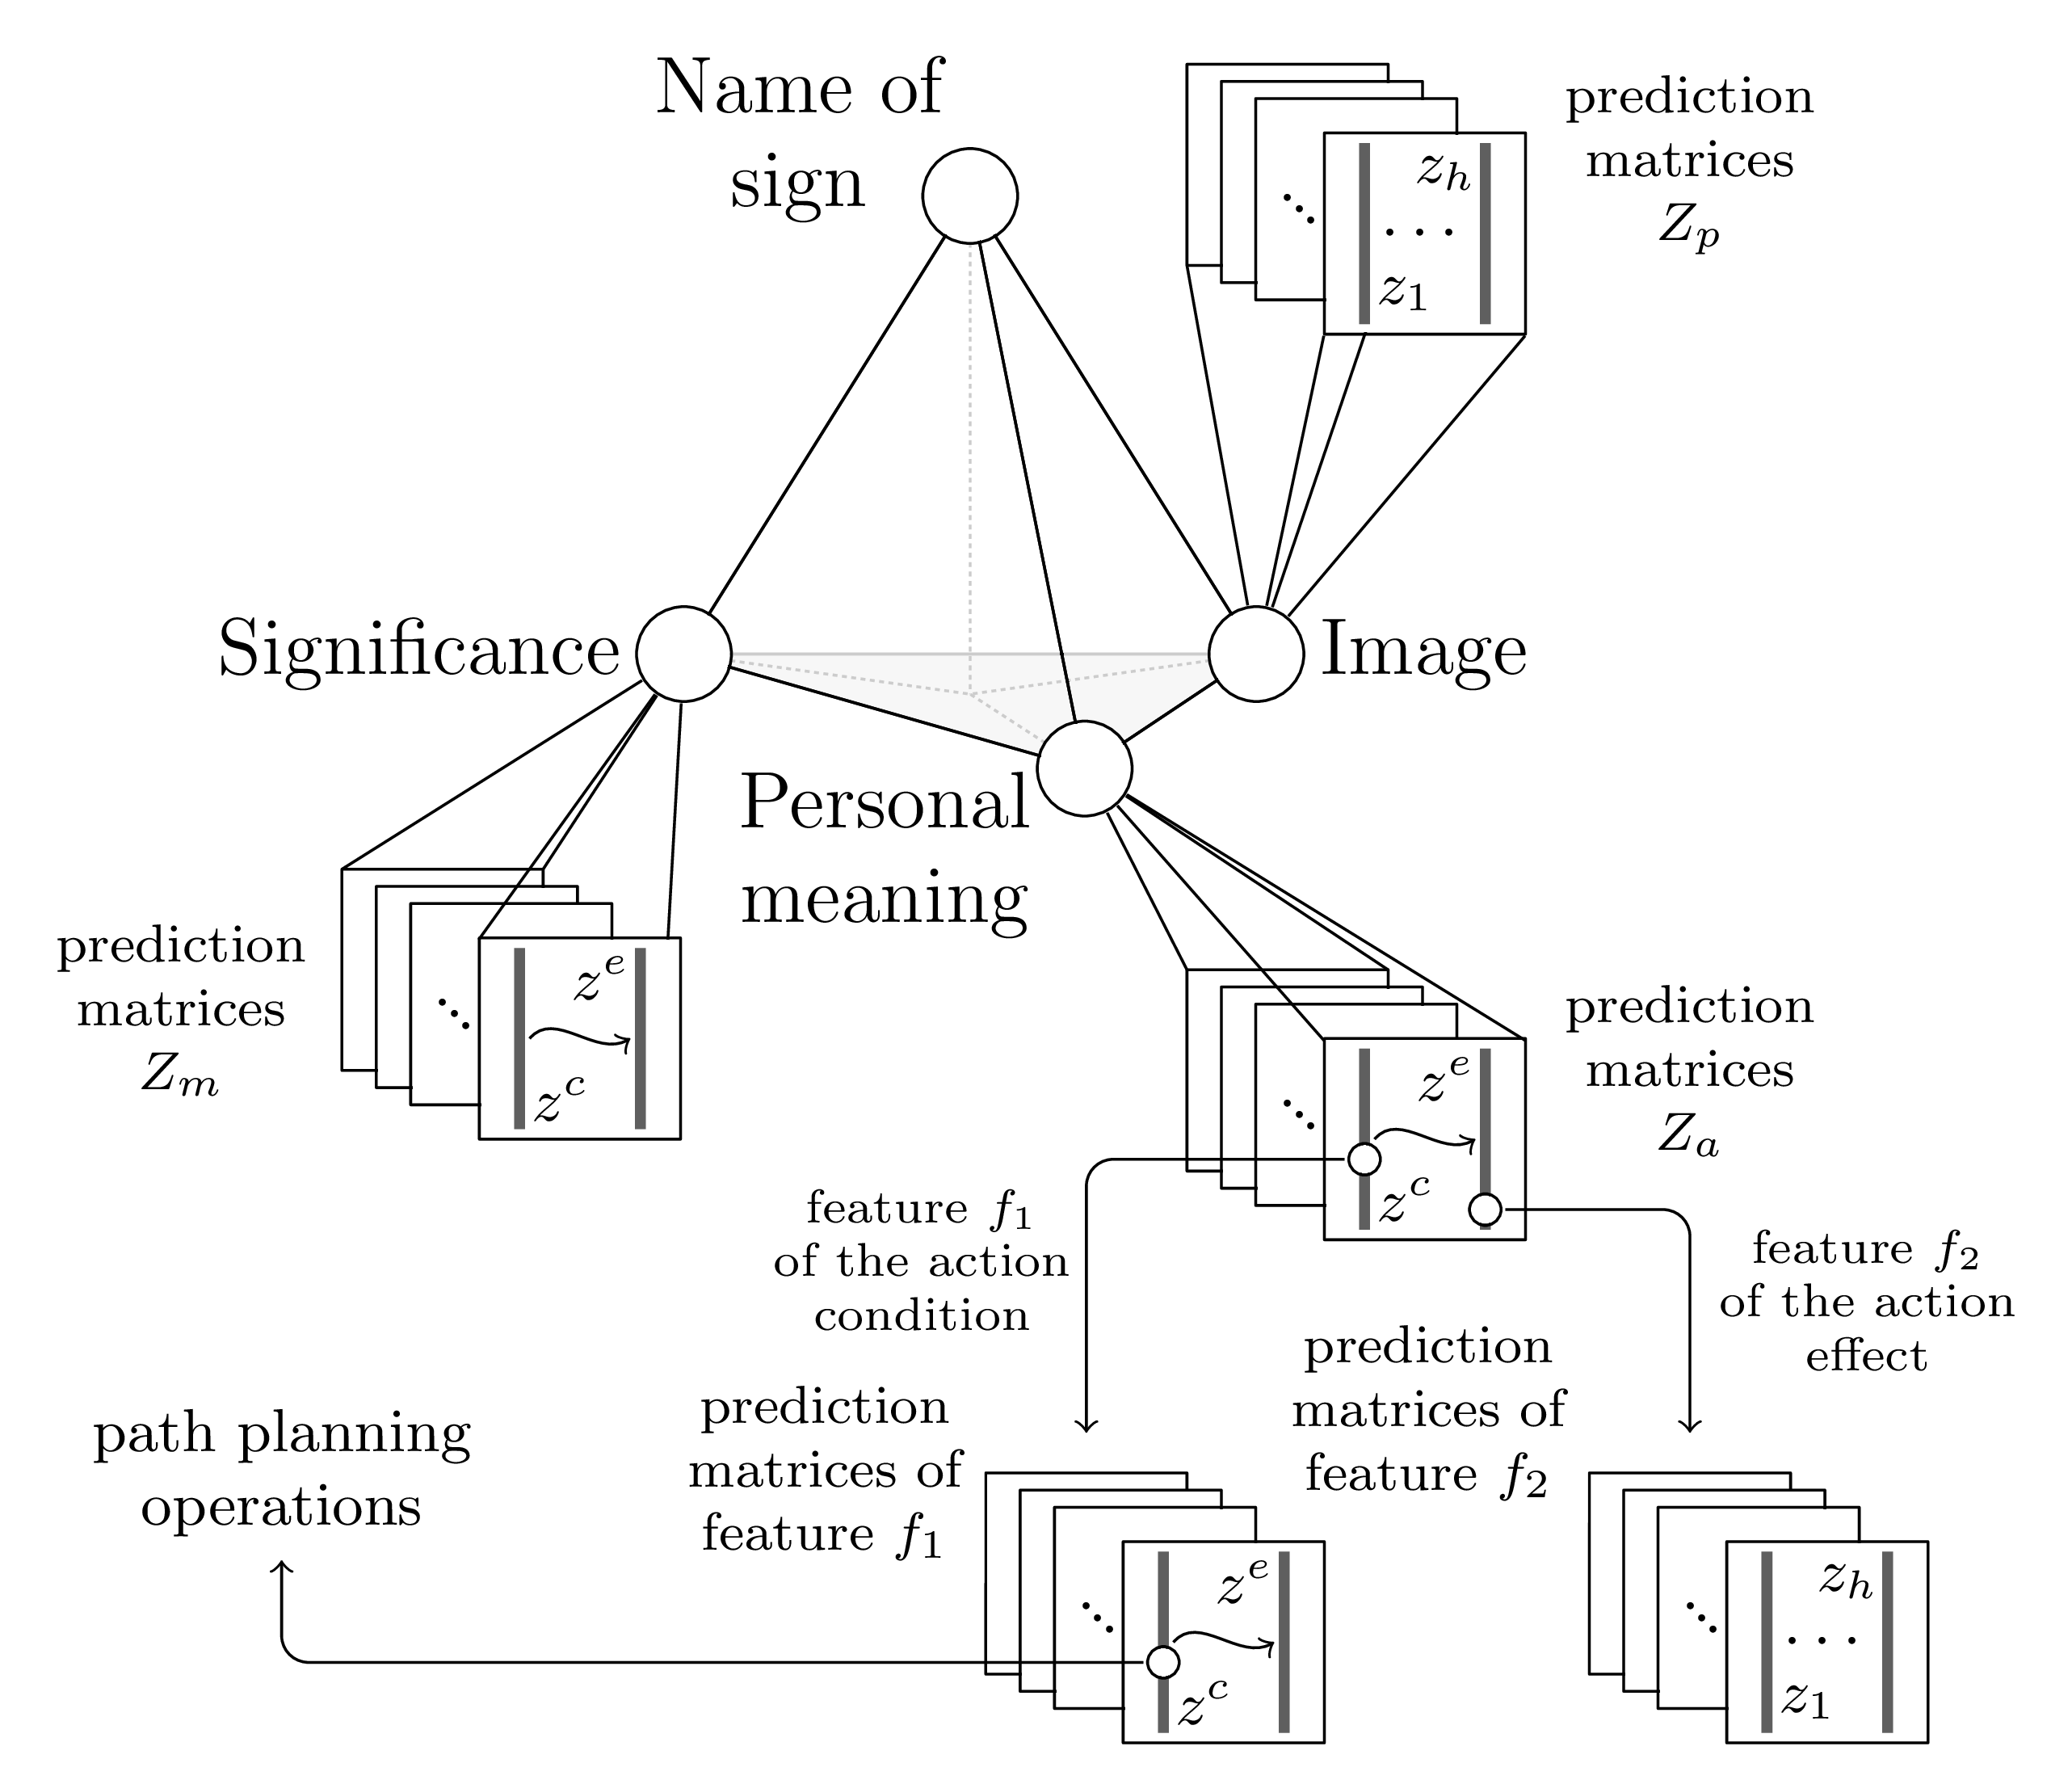
\includegraphics[width=0.8\textwidth]{signs/sign_kr.png}
			\end{column}
		\end{columns}
		
		This structure is supported by neuropsychological data (Edelmen, Ivanitsky, George, Hawkins etc.)
		
	\end{frame}

	\begin{frame}
		\frametitle{Sign world model}
		
		\begin{columns}
			\begin{column}{0.55\textwidth}
				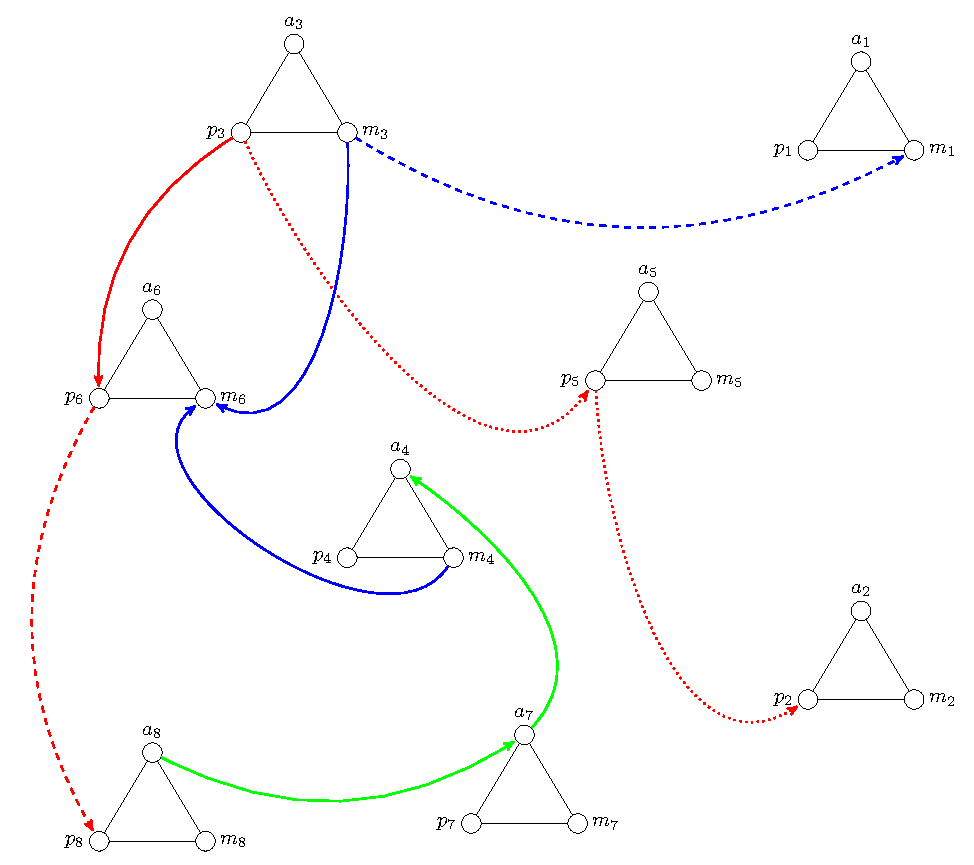
\includegraphics[width=\textwidth]{signs/signs_net}
			\end{column}
			\begin{column}{0.45\textwidth}
				\textit{Semiotic network} $H=\langle H_P, H_A, H_M\rangle$ consisting of three semantic network: 
				\begin{itemize}
					\item $H_P=\langle2^P,\mathfrak R_P\rangle$ -- semantic network on the set of sign images,
					\item $H_P=\langle2^A,\mathfrak R_A\rangle$ -- semantic network on the set of sign meanings,
					\item $H_P=\langle2^M,\mathfrak R_M\rangle$ -- semantic network on the set of sign significances.
				\end{itemize}
			\end{column}
		\end{columns}
	\end{frame}				

	\begin{frame}
		\frametitle{Behavior planning algorithm}
		
		\begin{columns}
			\begin{column}{0.7\textwidth}
				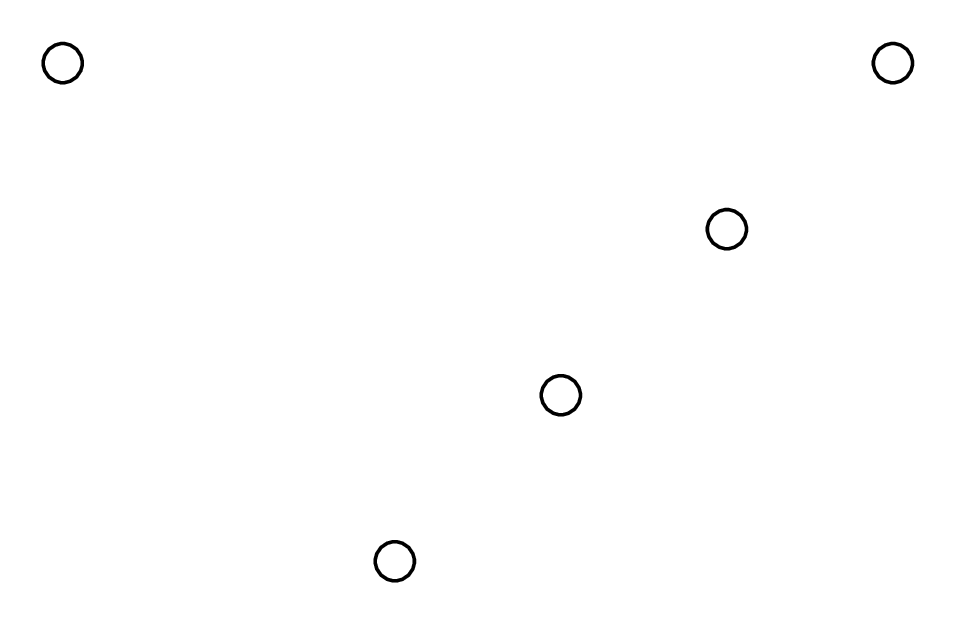
\includegraphics[width=\textwidth]{strl/beh_plan-0.png}
			\end{column}
			\begin{column}{0.3\textwidth}
				\tiny
				Planning starts from final situation and aims to meet start situation.
				\par\bigskip
				Main steps of algorithm (PMA iteration):
				\begin{itemize}
					\item \textit{M-step} -- search of relevant significances,
					\item \textit{A-step} -- choose a personal meaning from the set of personal meanings corresponding to the found significances,
					\item \textit{P-step} -- construct the new current situation using the set of features from the condition of performed action,
					\item \textit{S-step} -- send a message to other members of the coalition  or perform the action corresponding to the chosen personal meaning or execute action hierarchy up to \color{red} path planning operations.
				\end{itemize}
			\end{column}
		\end{columns}
	\end{frame}	

	\begin{frame}
		\frametitle{Path planning as graph search}
		
		\begin{columns}
			\begin{column}{0.55\textwidth}
				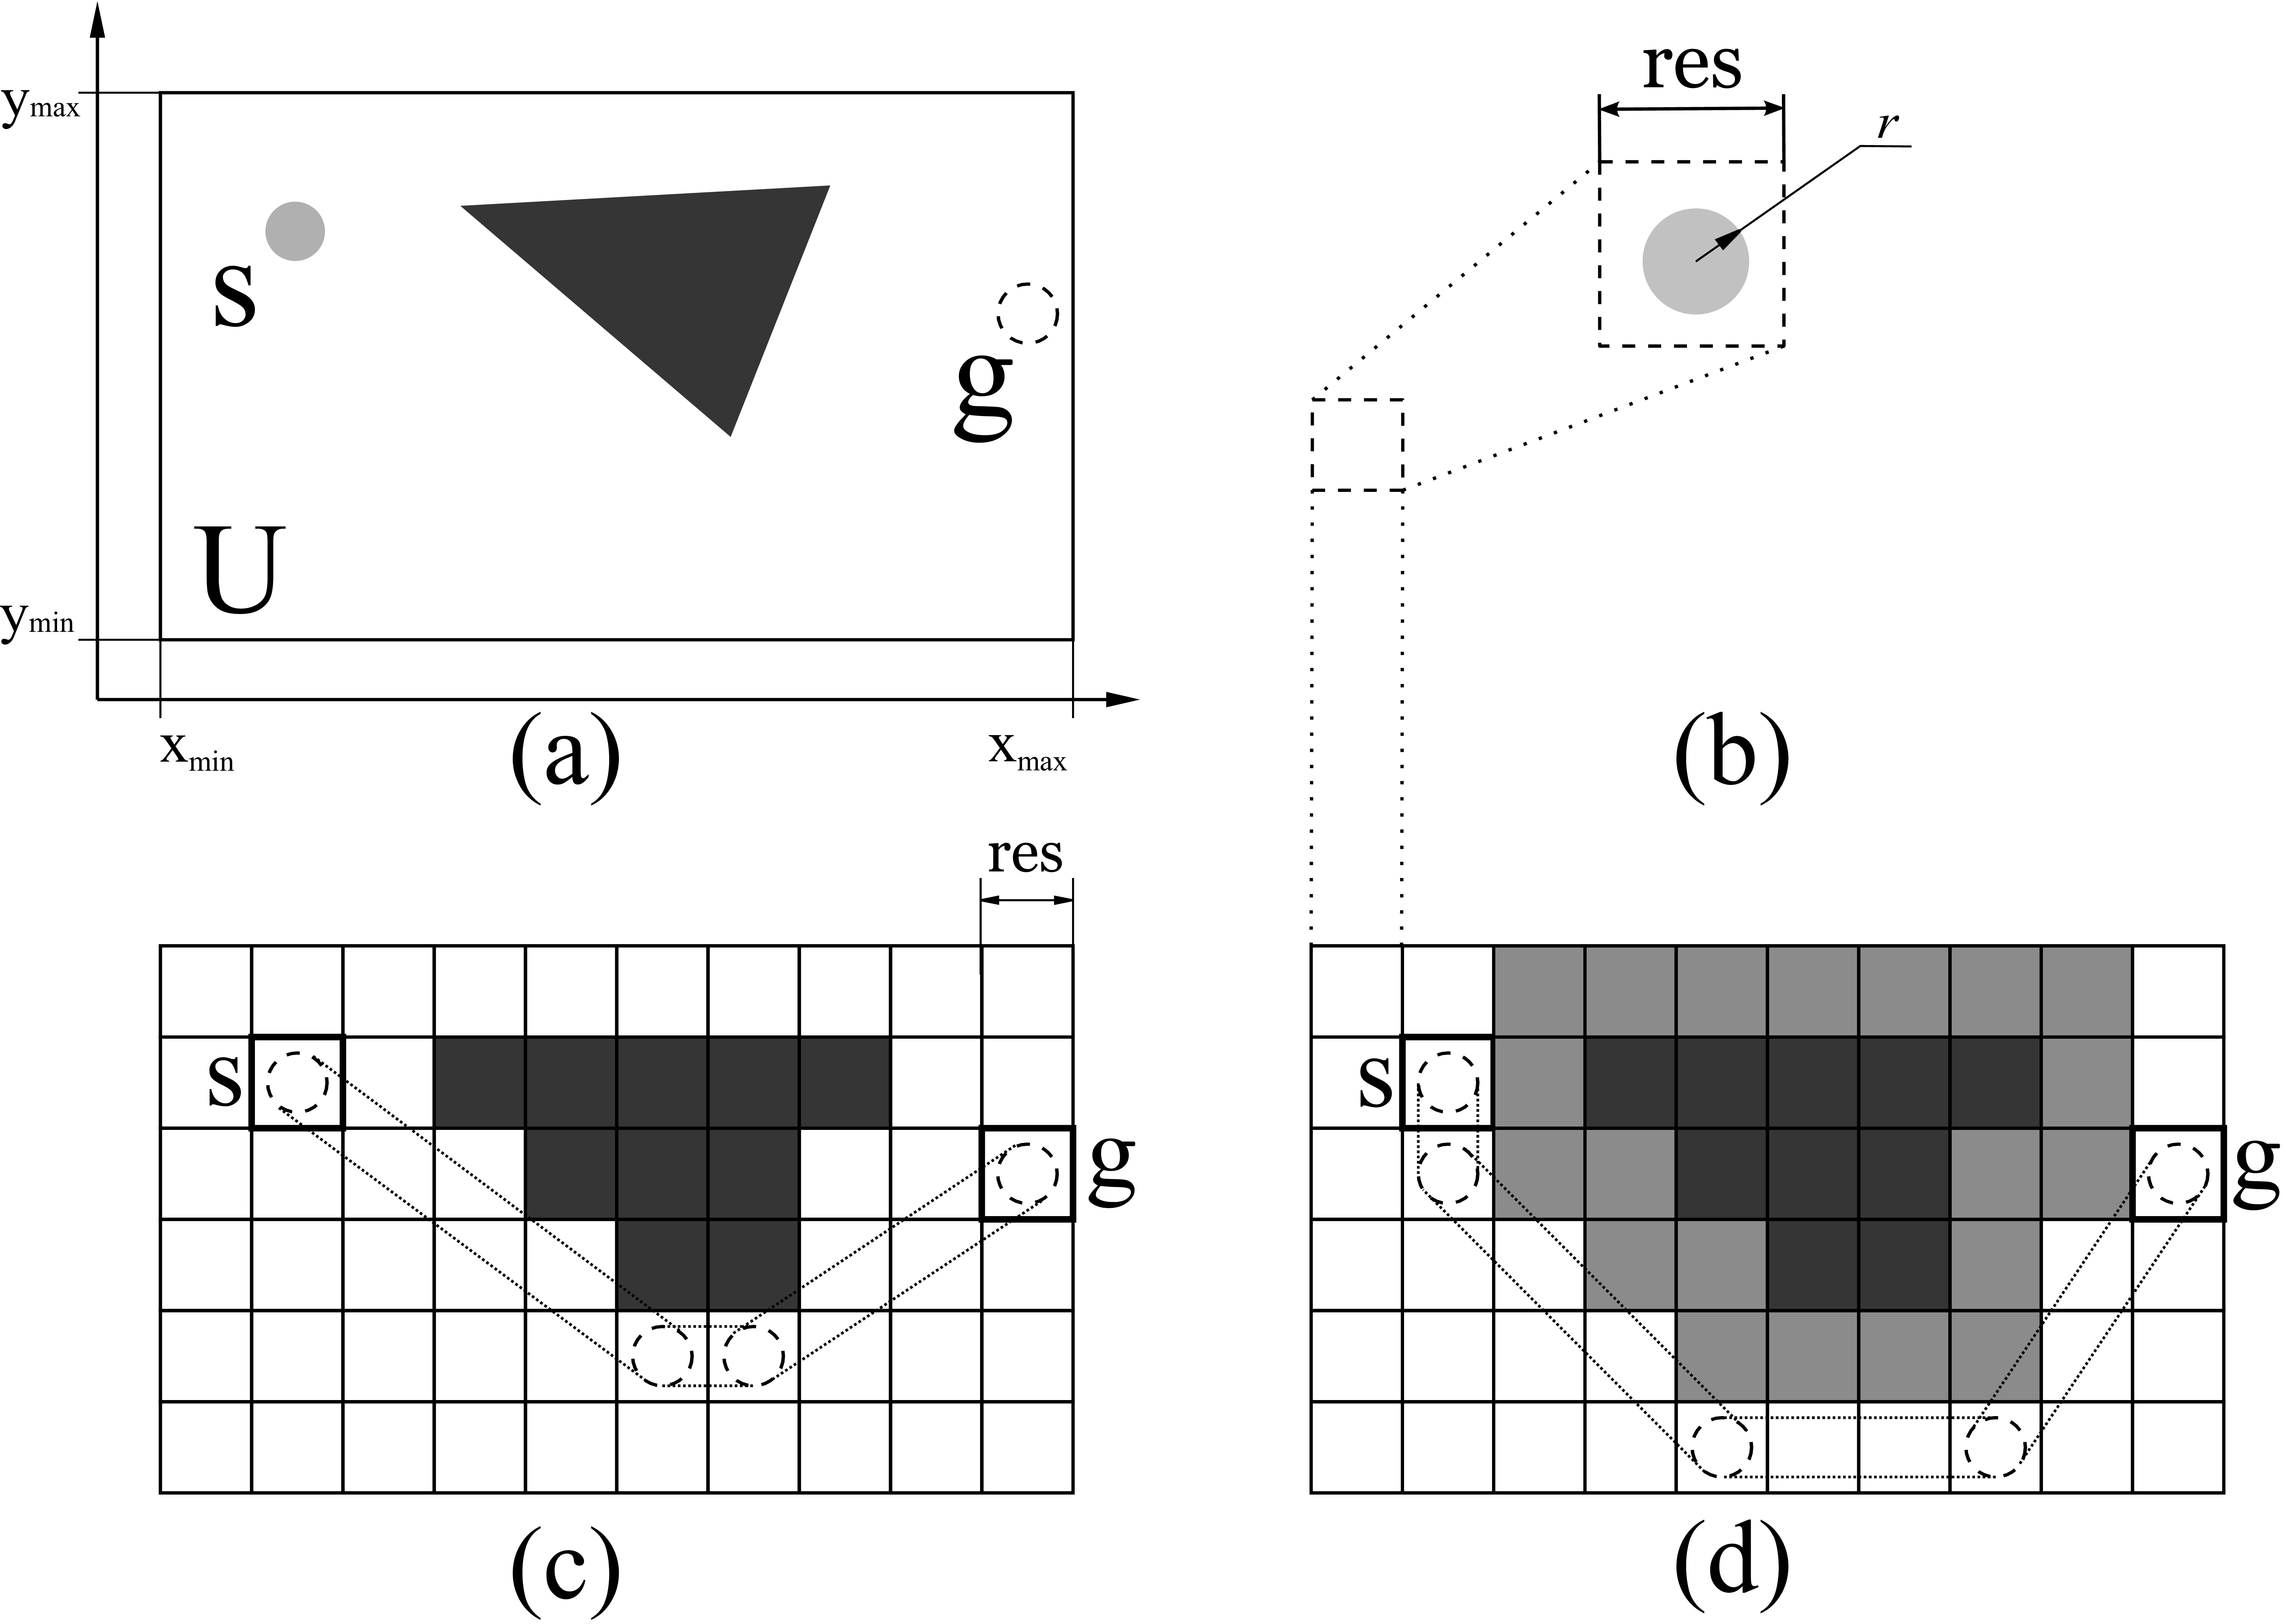
\includegraphics[width=\textwidth]{strl/path_grid.png}
			\end{column}
			\begin{column}{0.45\textwidth}
				\begin{minipage}[t][.6\textheight]{\textwidth}
					\textbf{Regular square grid} -- simple, informative and \textbf{easy-to-construct} spatial graph model for 2D path planning
					\vfill

					\fontsize{6}{7.2}\selectfont
					\textbf{Elfes, A. 1989.} Using occupancy grids for mobile robot perception and navigation. Computer, 22(6), 46-57.
					\par\medskip
					\textbf{Yap, P. 2002.} Grid-based path-finding. In Proceedings of 15th Conference of the Canadian Society for Computational Studies of Intelligence, 44-55. Springer Berlin Heidelberg.
					\par\medskip
					\textbf{Tozour, P. 2004.} Search space representations. In Rabin, S. (Ed.), AI Game Programming Wisdom 2, 85–102. Charles River Media.
				\end{minipage}
			\end{column}
		\end{columns}
	\end{frame}

	\begin{frame}
		\frametitle{Taking agent’s dynamic constraints into account}
		
		\begin{columns}
			\begin{column}{0.45\textwidth}
				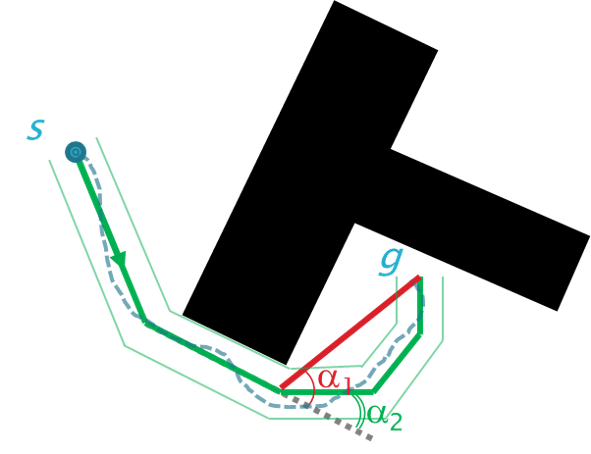
\includegraphics[width=0.8\textwidth]{strl/angl_constr_planning.png}
				\par\bigskip
				Angle-constrained path planning
			\end{column}
			\begin{column}{0.55\textwidth}
				Pure geometrical approach allows to state within compact, spatial-only search space (in contrary to “directly enhance the search-space with agent’s dynamic constraints” approach)
				\par\bigskip
				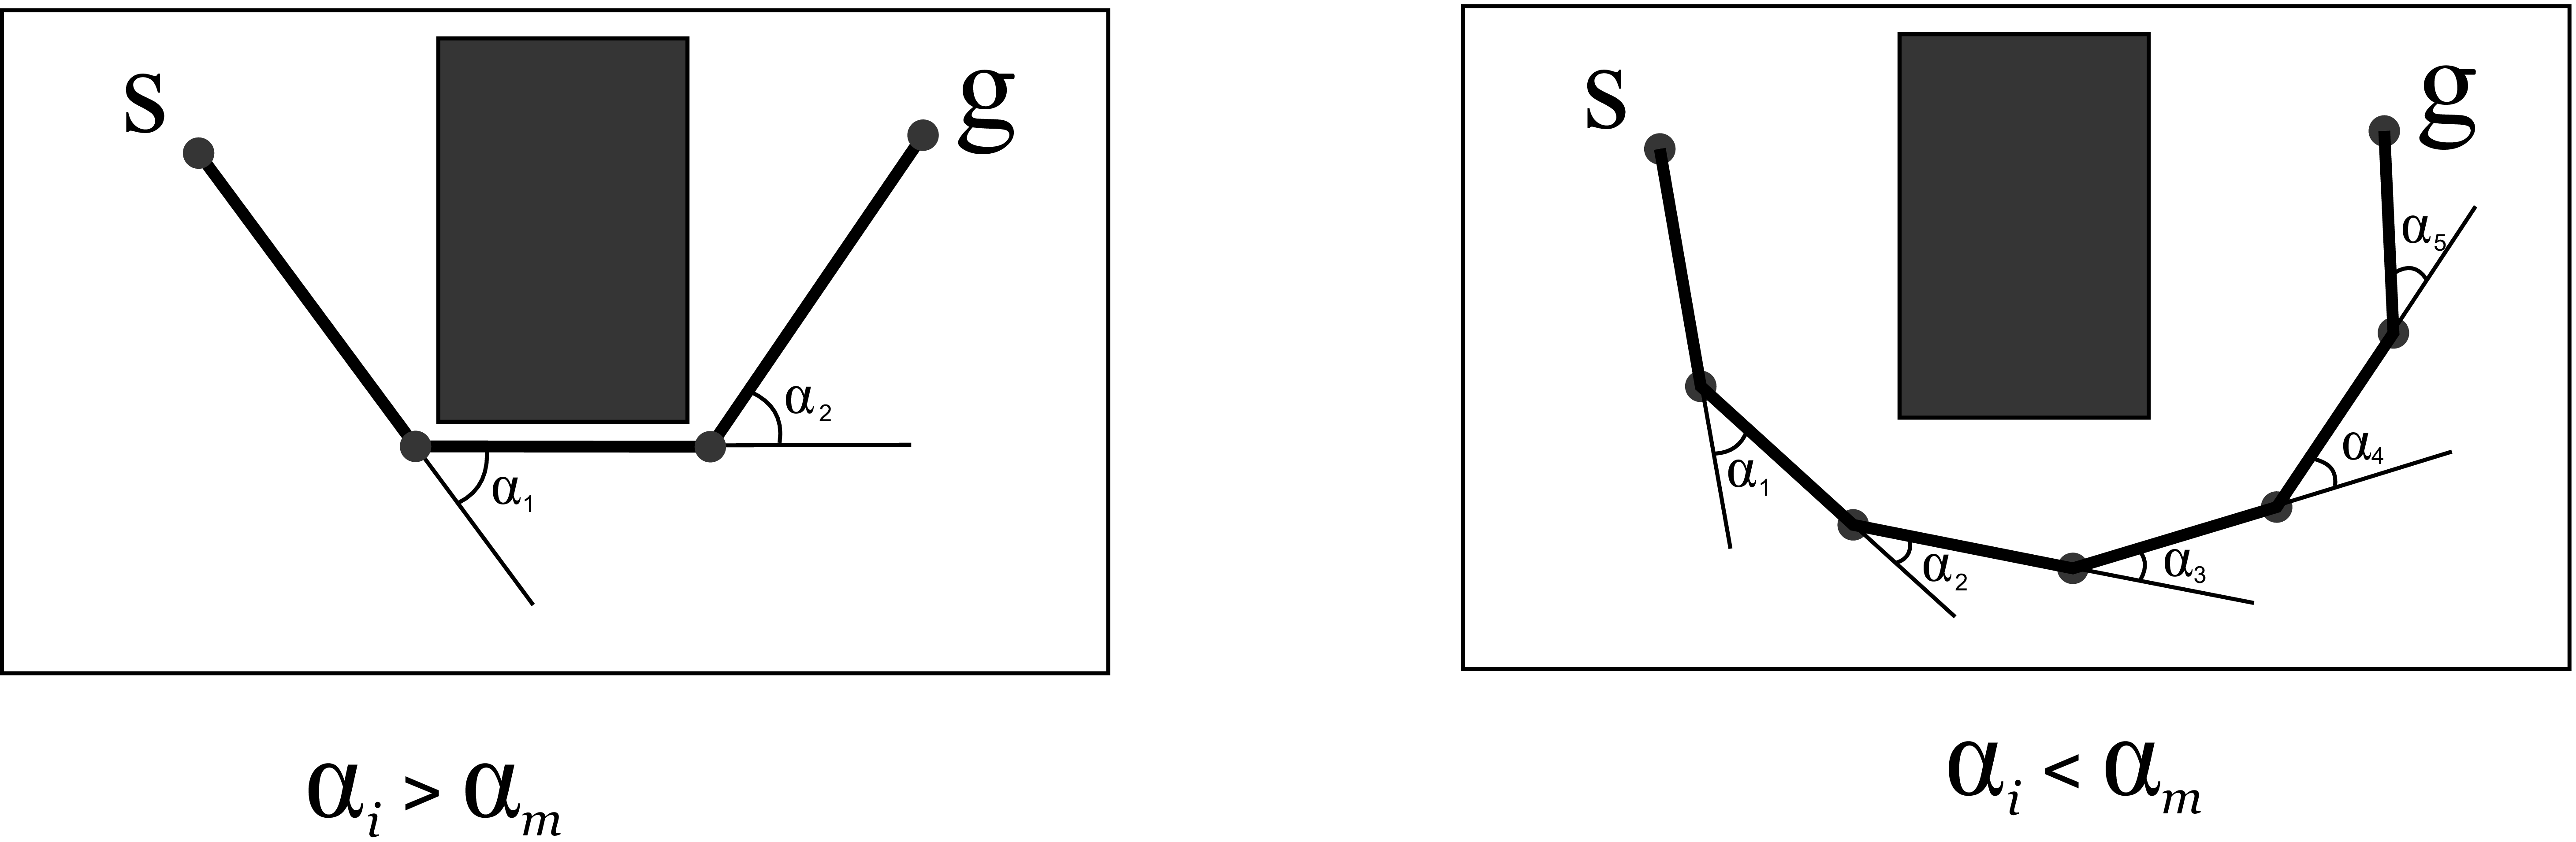
\includegraphics[width=\textwidth]{strl/path_lian.png}
			\end{column}
		\end{columns}
	\end{frame}

	\begin{frame}
		\frametitle{2 phases of path planning}

		\begin{minipage}[t][.6\textheight]{\textwidth}		
			\begin{enumerate}
				\item Path prediction (fast, no angle constraints)
				\begin{itemize}
					\item Using Theta* to find a path
					\item Use this path to calculate angle constraints (on reactive level)
				\end{itemize}
				\item Angle constrained path planning
				\begin{itemize}
					\item Using LIAN to find a path
					\begin{itemize}
						\item Not that fast
						\item No path can exist under constraint given
					\end{itemize}
				\end{itemize}
			\end{enumerate}
			
			\vfill
			
			\fontsize{6}{7.2}\selectfont
			Theta*: \textbf{Nash, A., Daniel, K., Koenig, S., Felner, A. 2007.} Theta*: Any-Angle Path Planning on Grids. In Proceedings of the National Conference on Artificial Intelligence (Vol. 22, No. 2, p. 1177). Menlo Park, Calif.: AAAI Press.
			\par\medskip
			LIAN: \textbf{Yakovlev, K., Baskin, E., Hramoin, I. 2015.} Grid-based angle-constrained path planning. In Proceedings of 38th Annual German Conference on AI, Dresden, Germany, September 21-25, 2015 (pp. 208-221).
		\end{minipage}
	\end{frame}

	\begin{frame}
		\frametitle{Theta* and LIAN}
		
		\begin{columns}
			\begin{column}{0.5\textwidth}
				\centering
				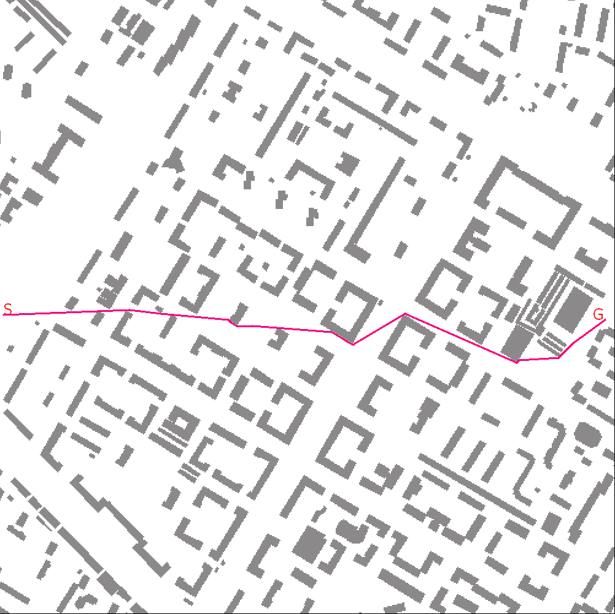
\includegraphics[width=0.9\textwidth]{misc/plan_theta.png}
			\end{column}
			\begin{column}{0.5\textwidth}
				\centering
				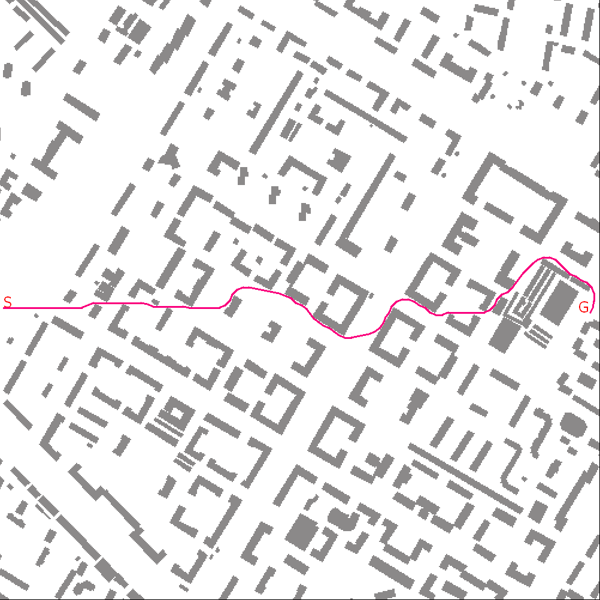
\includegraphics[width=0.9\textwidth]{misc/plan_lian.png}
			\end{column}
		\end{columns}
	\end{frame}

	\begin{frame}
		\frametitle{Interaction with Behavior planning}
		
		\begin{enumerate}
			\item Non-angle-constrained path can not be found
			\begin{itemize}
				\item It takes a while to come to that
				\item Identify blocking obstacle
				\item Pass id (or coordinates) of that obstacle to upper level of control
				\begin{itemize}
					\item On upper level: messaging for help, altering the coalition plan
				\end{itemize}
			\end{itemize}
			\item Non-angle-constrained path can is found but angle-constrained is not
			\begin{itemize}
				\item Agent can not reach goal area under current constraints (time, speed etc.)
				\item Inform upper level of control and ask for a task update (setting new time constraints for example)
			\end{itemize}
		\end{enumerate}
	\end{frame}

	\begin{frame}
		\frametitle{Case study}
		
		\begin{center}
			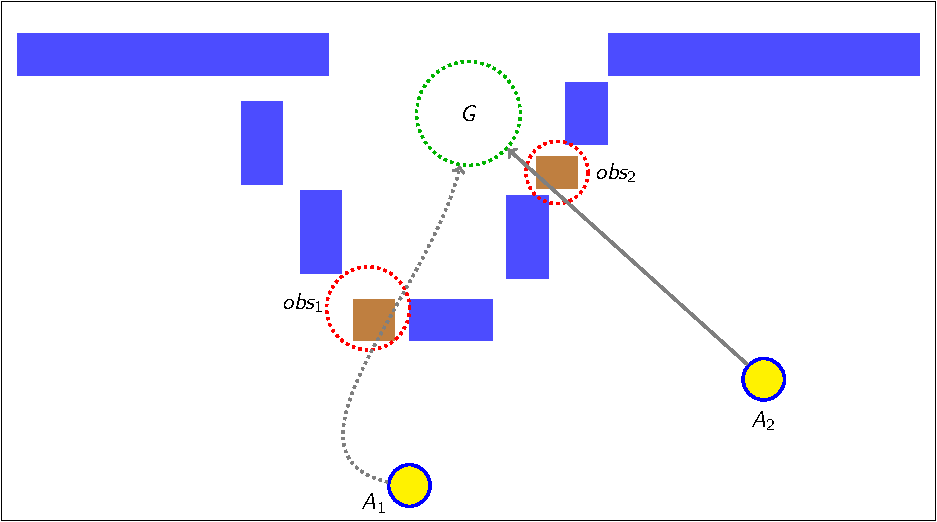
\includegraphics[page=1,width=0.85\textwidth]{slides_colored}
		\end{center}
		\par\bigskip
		Activated signs for agent $A_1$: ``place $X_6$'', ``far'', ``move 1'' $\rightarrow$ \color{red} path planning operations
	\end{frame}
	
	\begin{frame}
		\frametitle{Case study}
		
		\begin{center}
			\includegraphics[page=31,width=0.85\textwidth]{slides_colored}
		\end{center}
		\par\bigskip
		Activated signs for agent $A_1$: ``obstacle 1'', ``near'', ``place $X_6$''
	\end{frame}

	\begin{frame}
		\frametitle{Case study}
		
		\begin{center}
			\includegraphics[page=42,width=0.85\textwidth]{slides_colored}
		\end{center}
		\par\bigskip
		Activated signs for agent $A_1$: ``send message'', ``agent $A_2$''
	\end{frame}

	\begin{frame}
		\frametitle{Case study}
		
		\begin{center}
			\includegraphics[page=58,width=0.85\textwidth]{slides_colored}
		\end{center}
		\par\bigskip
		Activated signs for agent $A_2$: ``place $Y_3$'', ``far'', ``move 2'' $\rightarrow$ \color{red} path planning operations
	\end{frame}

	\begin{frame}
		\frametitle{Case study}
		
		\begin{center}
			\includegraphics[page=95,width=0.85\textwidth]{slides_colored}
		\end{center}
		\par\bigskip
		Activated signs for agent $A_2$: ``place $Y_1$'', ``near'', ``obstacle 1'', ``destroy''
	\end{frame}

	\begin{frame}
		\frametitle{Case study}
		
		\begin{center}
			\includegraphics[page=116,width=0.85\textwidth]{slides_colored}
		\end{center}
		\par\bigskip
		Activated signs for agents $A_1$ and $A_2$: ``far'', ``move 3'' $\rightarrow$ \color{red} path planning operations
	\end{frame}

	\begin{frame}
		\frametitle{Case study}
		
		\begin{center}
			\includegraphics[page=171,width=0.85\textwidth]{slides_colored}
		\end{center}
		\par\bigskip
		Activated signs for agents $A_1$ and $A_2$: goal state (``place G'')
	\end{frame}
					
	\begin{frame}
		\frametitle{Summary}
		\begin{itemize}
			\item Special type of navigation tasks (smart relocation tasks) 
			\item New method for knowledge representation -- sign world model based on psychological and neurophysiological data
			\item Top-level PMA planner (behavior planner) -- iterative search procedure in semiotic network
			\item Path planner resides on the lowest level of behavior planner hierarchy
			\item 2 phase path planning: path prediction (fast) path planning taking into account agent’s dynamic constraints (slow)
		\end{itemize}
		\par\bigskip
		\textbf{Future work}
		\begin{itemize}
			\item Path planning
			\begin{itemize}
				\item WHY we can not find a path (blocking obstacles, tough constraints etc)
			\end{itemize}
			\item Behavior planning
			\begin{itemize}
				\item Investigation of time and space special constraints
			\end{itemize}
		\end{itemize}
		
	\end{frame}
								
	\begin{frame}
		\centering
		\Huge
		Questions?
		\normalsize
		\par\bigskip
		\par\bigskip
		Russian Academy of Sciences, pan@isa.ru, yakovlev@isa.ru
	\end{frame}
									
	%	\begin{frame}
	%		\frametitle{Цели курса}
	%		
	%		\begin{itemize}
	%			\item
	%		\end{itemize}
	%	\end{frame}
	
\end{document}
	
	
